\documentclass[12pt,a4paper]{article}
\usepackage[margin=1in]{geometry}
\usepackage[T1]{fontenc}
\usepackage[utf8]{inputenc}
\usepackage{lmodern,microtype}
\usepackage{setspace,graphicx,xcolor,booktabs,longtable,array,enumitem,hyperref,fancyhdr,titlesec,tikz}
\usetikzlibrary{arrows.meta,positioning,shapes.geometric}
\definecolor{navy}{HTML}{102A43}
\definecolor{teal}{HTML}{147D92}
\definecolor{pale}{HTML}{F0F5F9}
\hypersetup{colorlinks=true,linkcolor=navy,urlcolor=teal,pdftitle={OMNISENT Project Proposal}}
\titleformat{\section}{\Large\bfseries\color{navy}}{\thesection}{0.7em}{}
\titleformat{\subsection}{\large\bfseries\color{teal}}{\thesubsection}{0.7em}{}
\pagestyle{fancy}\fancyhf{}\lhead{\textcolor{navy}{OMNISENT}}\rhead{\textcolor{navy}{Project Proposal}}\cfoot{\thepage}
\setlength{\headheight}{15pt}\setstretch{1.12}
\begin{document}
\begin{titlepage}\centering\vspace*{1.1cm}
{\Large\bfseries PROJECT PROPOSAL\par}\vspace{0.8cm}
{\Huge\bfseries\color{navy} OMNISENT\par}\vspace{0.25cm}
{\Large Hybrid Robotic Surveillance \& Autonomous Exploration Platform\par}\vspace{0.8cm}

\begin{tikzpicture}
\draw[teal,line width=1.5pt,rounded corners=8pt] (0,0) rectangle (10,2.1);
\node[font=\Large\bfseries,text=navy] at (5,1.3) {OMNISENT};
\node[font=\small,text=teal] at (5,0.7) {SENSE \textbullet\ CONNECT \textbullet\ OBSERVE};
\end{tikzpicture}\vspace{1cm}
\begin{tabular}{>{\bfseries}p{4cm}p{7cm}}
Student Name: & [Insert name] \\
Student ID: & [Insert ID] \\
Course Title: & [Insert course title] \\
Course Code: & [Insert course code] \\
Submitted To: & [Instructor name/designation] \\
Department: & [Insert department] \\
Institution: & [Insert institution] \\
Submission Date: & [Insert date] \\
\end{tabular}
\vfill{\large Initial proposal and design artefacts\par}\end{titlepage}
\pagenumbering{roman}\tableofcontents\newpage\pagenumbering{arabic}

\section{Executive Summary}
OMNISENT is a proposed modular robotic surveillance and remote-control platform intended to combine a ground robot, a structured software application, and extensible observation services. The initial academic prototype will focus on remote command handling, connection/status reporting, mission records, and a Java-based control interface. The proposed architecture combines Java application logic, Python-based voice/camera services, an ESP8266 communication bridge, and an Arduino-compatible embedded controller.

The project demonstrates object-oriented programming, modular design, interfaces, networking, data modelling, requirements analysis, testing, and version control. Server-side mission storage and phone-friendly status access are design goals whose implementation will depend on deployment and network decisions. Drone-assisted observation, improved localization, obstacle avoidance, and mapping are future research directions—not initial deliverables.

\section{Introduction}
A useful robotic vehicle requires more than movement: it needs clear operator controls, reliable communication, status feedback, structured mission records, and maintainable software. OMNISENT proposes separating the operator-facing application, optional voice/camera services, communication bridge, embedded control, and data model so components can be tested independently and extended over time.

\section{Problem Statement}
A basic remote-controlled or line-following robot may lack a unified application for mission management, command history, status reporting, and future service integration. A system tightly coupled to a prepared track may also be limited when the environment changes. Unstructured logs and unclear software boundaries can make debugging and future development difficult. OMNISENT addresses these concerns through a modular design, a defined communication boundary, mission/event records, and a roadmap for improved sensing and navigation. The initial prototype will not claim full autonomy.

\section{Aim and Objectives}
\subsection{General Aim}
To design and prototype a modular robotic surveillance and remote-control platform while demonstrating software engineering and Java object-oriented programming principles.
\subsection{Specific Objectives}
\begin{enumerate}
\item Design a Java application for command coordination and mission management.
\item Define a communication interface between the application and ESP8266/Arduino controller.
\item Provide a simple interface for movement commands and status display.
\item Plan integration with existing Python voice-recognition and camera services.
\item Model mission records, command events, and captured-image references.
\item Produce DFD, use case, activity, ERD, class, and object diagrams.
\item Define a development schedule, milestones, deliverables, and verification plan.
\item Establish a future path for localization, obstacle avoidance, mapping, and drone-assisted observation.
\end{enumerate}

\section{Scope}
\subsection{Initial scope}
Requirements analysis, architecture, six design diagrams, a Java prototype using at least five classes, a simple interface, a proposed data model, testing plan, and GitHub documentation. The prototype should use a mock communication adapter before physical integration.
\subsection{Out of scope}
Fully autonomous navigation in arbitrary environments, completed drone flight control, full humanoid mechanics, and verified GPS/localization without appropriate hardware. No capability will be described as tested unless it has actually been tested.

\section{Proposed Features}
\subsection{Core features}
\begin{itemize}
\item Command model for forward, backward, left, right, and stop.
\item Connection-state and robot-status representation.
\item Mission creation, completion, and history.
\item Command/event logging with timestamps.
\item Java interface backed by testable domain classes.
\item Planned integration boundaries for Python voice and camera services.
\end{itemize}
\subsection{Planned remote access}
Phone-friendly status access and server-side data storage are proposed. They require a defined API, deployment decision, authentication, and network testing. Geographic location display requires a suitable position source; GPS must not be claimed without compatible hardware and integration.

\section{Stakeholders}
The operator issues commands and reviews status. The developer implements, tests, and documents the application. The course instructor evaluates design artefacts and Java concepts. Future maintainers may add sensors, services, or autonomy modules.

\section{Functional Requirements}
\begin{longtable}{p{1.2cm}p{9cm}p{2cm}}\toprule
ID & Requirement & Priority\\\midrule
FR-01 & Provide an operator interface for robot commands. & Must\\
FR-02 & Represent forward, backward, left, right, and stop commands. & Must\\
FR-03 & Represent connection state and report communication errors. & Must\\
FR-04 & Send commands through a defined communication adapter. & Must\\
FR-05 & Represent status received from the robot controller. & Must\\
FR-06 & Create mission records with identifiers, timestamps, and status. & Must\\
FR-07 & Associate command/event records with missions. & Should\\
FR-08 & Support a replaceable camera-capture service. & Should\\
FR-09 & Allow integration with Python voice/vision services. & Should\\
FR-10 & Allow future server-side storage and phone-friendly status access. & Future\\
FR-11 & Allow future localization, obstacle avoidance, mapping, and drone integration. & Future\\\bottomrule
\end{longtable}

\section{Non-Functional Requirements}
\begin{itemize}
\item \textbf{Maintainability:} clear, cohesive class responsibilities.
\item \textbf{Extensibility:} interfaces isolate service implementations.
\item \textbf{Reliability:} timeouts and explicit error states.
\item \textbf{Usability:} clear controls and connection state.
\item \textbf{Safety:} stop behaviour and safe motor state considered before hardware tests.
\item \textbf{Security:} authentication and access control before remote deployment.
\item \textbf{Data integrity:} consistent identifiers and timestamps.
\item \textbf{Testability:} core logic testable without physical hardware.
\end{itemize}

\section{Proposed Architecture}
The architecture separates six responsibilities: (1) Java presentation layer, (2) Java application layer, (3) Python voice/camera services, (4) communication interface and ESP8266 bridge, (5) Arduino C/C++ embedded control, and (6) mission/event data storage.
\begin{figure}[htbp]\centering
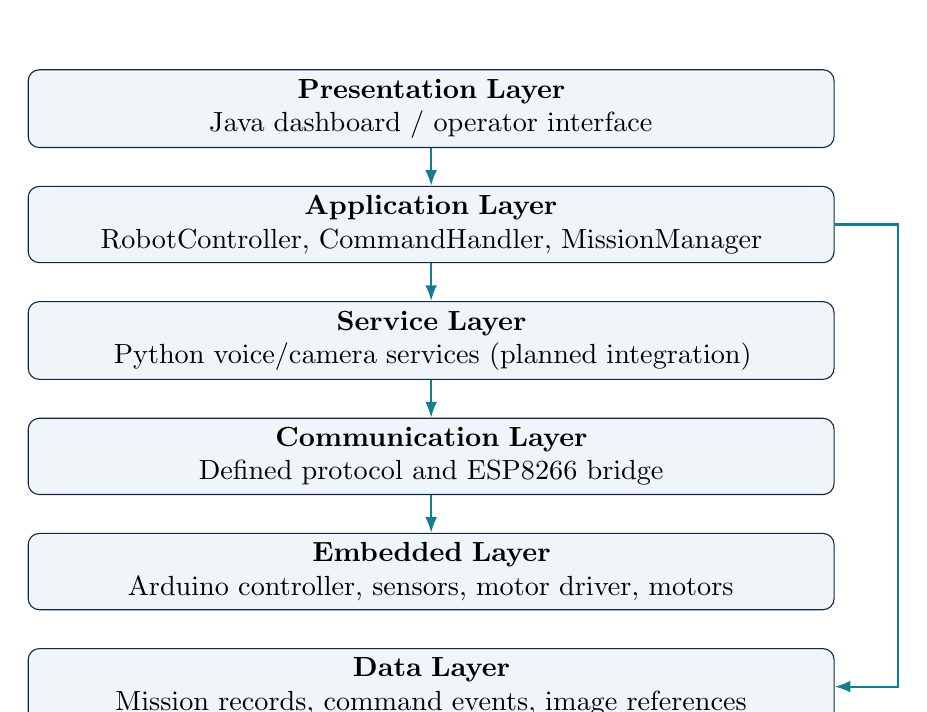
\begin{tikzpicture}[node distance=0.48cm,block/.style={draw=navy,fill=pale,rounded corners=4pt,align=center,text width=10cm,minimum height=0.75cm},arr/.style={-{Latex[length=2mm]},thick,color=teal}]
\node[block] (ui) {\textbf{Presentation Layer}\\Java dashboard / operator interface};
\node[block,below=of ui] (app) {\textbf{Application Layer}\\RobotController, CommandHandler, MissionManager};
\node[block,below=of app] (py) {\textbf{Service Layer}\\Python voice/camera services (planned integration)};
\node[block,below=of py] (net) {\textbf{Communication Layer}\\Defined protocol and ESP8266 bridge};
\node[block,below=of net] (hw) {\textbf{Embedded Layer}\\Arduino controller, sensors, motor driver, motors};
\node[block,below=of hw] (data) {\textbf{Data Layer}\\Mission records, command events, image references};
\draw[arr] (ui)--(app);\draw[arr] (app)--(py);\draw[arr] (py)--(net);\draw[arr] (net)--(hw);\draw[arr] (app.east)--++(0.8,0)|-(data.east);
\end{tikzpicture}
\caption{Proposed logical architecture; this is not a finalized protocol specification.}
\end{figure}

\section{Technology Stack}
\begin{longtable}{p{3cm}p{4cm}p{5.2cm}}\toprule
Area & Proposed technology & Role\\\midrule
Main application & Java & OOP, command model, mission management\\
Interface & JavaFX or Swing & Operator controls and status\\
Networking & Java TCP sockets / HTTP API & Communication with services and bridge\\
Voice/vision & Python & Existing recognition and camera functions\\
Embedded firmware & Arduino C/C++ & Sensors and low-level motor control\\
Wireless bridge & ESP8266 & Network-to-serial bridge\\
Persistence & JSON initially; relational database if needed & Mission/event records\\
Diagrams & Mermaid and PlantUML & Design sources\\
Documentation & LaTeX & Formal proposal PDF\\
Version control & Git and GitHub & Change history and submission\\\bottomrule
\end{longtable}

\section{Java Class Design}
The proposed design includes \texttt{RobotController}, \texttt{CommandHandler} (interface), \texttt{ConnectionManager} (interface), \texttt{MockConnectionManager}, \texttt{MissionManager}, \texttt{MissionRecord}, \texttt{RobotDashboard}, \texttt{CommandResult}, and \texttt{RobotStatus}. The class diagram is maintained in \texttt{diagrams/class-diagram.mmd}. The prototype must use at least five diagrammed classes; listing names alone does not satisfy the interface requirement.

\section{Software Process Model}
An iterative and incremental model is proposed:
\begin{enumerate}
\item Requirements and feasibility.
\item Architecture and UML design.
\item Java domain model and simple interface.
\item Command adapter and mock-based tests.
\item Python-service and hardware integration after protocol confirmation.
\item Verification, documentation, and evaluation.
\end{enumerate}

\section{Schedule, Milestones, and Deliverables}
The Gantt source is maintained in \texttt{diagrams/gantt.mmd}. The schedule is illustrative and must be aligned with the actual course deadline.
\begin{longtable}{p{1.2cm}p{3.5cm}p{5.5cm}p{2cm}}\toprule
ID & Milestone & Deliverable & Evidence\\\midrule
M1 & Proposal baseline & Proposal and requirements & Scope documented\\
M2 & Design baseline & Six diagrams & Consistency review\\
M3 & Java prototype & Interface and five or more classes & Source and demonstration\\
M4 & Communication proof & Mock/controlled command exchange & Test record\\
M5 & Final evaluation & Documentation and repository & Limitations and outcomes reported\\\bottomrule
\end{longtable}

\section{Data Model}
The proposed relational model contains \texttt{OPERATOR}, \texttt{ROBOT}, \texttt{MISSION}, \texttt{COMMAND\_EVENT}, and \texttt{CAPTURED\_IMAGE}. A mission is associated with an operator and robot and may have multiple command events and captured-image references. This is a proposed design; JSON may be used in the initial prototype before a database is required.

\section{Testing and Evaluation}
\begin{longtable}{p{1.2cm}p{5cm}p{6cm}}\toprule
ID & Test & Expected evidence\\\midrule
T-01 & Validate supported and invalid commands & Correct result or validation error\\
T-02 & Test controller with mock adapter & Command and result represented\\
T-03 & Simulate disconnect/timeout & Error state shown; application remains responsive\\
T-04 & Create and close mission & Consistent ID, timestamps, and status\\
T-05 & Retrieve mission history & Existing records returned\\
T-06 & Verify class usage & Five or more diagrammed classes used by the interface\\
T-07 & Test physical integration when ready & Controlled test record, not an assumption\\
T-08 & Test camera service when available & Image reference or explicit error\\\bottomrule
\end{longtable}

\section{Risks and Mitigation}
\begin{longtable}{p{3cm}p{4cm}p{5cm}}\toprule
Risk & Impact & Mitigation\\\midrule
Scope expansion & Core submission delayed & Keep drone as future work\\
Firmware/protocol mismatch & Integration failure & Confirm actual firmware and protocol\\
Network instability & Lost/delayed commands & Timeouts, validation, status display\\
Voice recognition noise & Unreliable voice control & Preserve manual control\\
Missing localization hardware & Position cannot be verified & Treat localization as conditional future work\\
Unsafe movement & Hardware/environment damage & Safe stop and controlled tests\\
Security gaps & Unauthorized access & Do not expose prototype without access control\\\bottomrule
\end{longtable}

\section{Future Work: Drone-Assisted Surveillance}
A future version may integrate a drone with the ground rover to provide aerial observation when a wider view is useful while the ground robot performs close-range inspection. This could form a coordinated ground-air surveillance platform. It would require separate work on flight hardware, communications, localization, battery management, operator control, and flight safety. Drone integration is therefore a long-term research direction, not an initial prototype commitment. Other possible extensions include LiDAR-assisted mapping, obstacle avoidance, improved localization, and a redesigned robotic body.

\section{Expected Deliverables}
\begin{enumerate}
\item Proposal and requirements specification.
\item Process model, milestones, deliverables, and Gantt chart.
\item Data Flow Diagram.
\item Use Case Diagram.
\item Activity Diagram.
\item Entity Relationship Diagram.
\item Class Diagram.
\item Object Diagram.
\item Java interface using at least five diagrammed classes.
\item Source files and GitHub repository.
\item Test plan and verified/planned functionality status.
\end{enumerate}

\section{Conclusion}
OMNISENT proposes a modular path toward robotic surveillance and remote control. Its initial academic contribution is a defined architecture and Java prototype supported by requirements, design diagrams, a schedule, and verification criteria. Separating application logic, optional Python services, communication, embedded control, and data should make the system easier to test and extend. Drone-assisted observation and advanced autonomy remain future work subject to feasibility and safety assessment.

\section{References}
\begin{itemize}
\item Oracle, \emph{Java Documentation}: \url{https://docs.oracle.com/en/java/}
\item Arduino, \emph{Arduino Documentation}: \url{https://docs.arduino.cc/}
\item Mermaid, \emph{Mermaid Documentation}: \url{https://mermaid.js.org/}
\item PlantUML, \emph{PlantUML Documentation}: \url{https://plantuml.com/guide}
\end{itemize}
\end{document}
